% Template for ICIP-2018 paper; to be used with:
%          spconf.sty  - ICASSP/ICIP LaTeX style file, and
%          IEEEbib.bst - IEEE bibliography style file.
% --------------------------------------------------------------------------
\documentclass{article}
\usepackage{res/packages/spconf,amsmath,graphicx}
\graphicspath{{res/imgs/},{res/plots/}}
\usepackage{hyperref}
\usepackage{url}
\newcommand{\link}[1]{\href{#1}{\textit{#1}}}
% Example definitions.
% --------------------
\def\x{{\mathbf x}}
\def\L{{\cal L}}

\renewcommand{\thesection}{\Roman{section}}
\renewcommand{\thesubsection}{\roman{subsection}}
\renewcommand{\thesubsubsection}{\alph{subsubsection}}


%prout


% Title.
% ------
\title{Website analyse : \textit{miniclip.com}}
%
% Single address.
% ---------------
\name{28681700
\thanks{Thanks to my mum.}}
\address{}
%
% For example:
% ------------
%\address{School\\
%	Department\\
%	Address}
%
% Two addresses (uncomment and modify for two-address case).
% ----------------------------------------------------------
%\twoauthors
%  {A. Author-one, B. Author-two\sthanks{Thanks to XYZ agency for funding.}}
%	{School A-B\\
%	Department A-B\\
%	Address A-B}
%  {C. Author-three, D. Author-four\sthanks{The fourth author performed the work
%	while at ...}}
%	{School C-D\\
%	Department C-D\\
%	Address C-D}
%
\begin{document}
%\ninept
%
\maketitle
%
\begin{abstract}
This report contains an analyzis of the website \link{miniclip.com}. The analyze covers three particular aspects: \textit{HTTP}, \textit{DNS} and \textit{TCP} packets.
\end{abstract}
%
% \begin{keywords}
% One, two, three, four, five
% \end{keywords}
%
\section{Introduction}
\label{sec:intro}
\subsection{Website}
\label{sub:web}
\textit{Minclip} is a free online games website. It was launched in 2001 by \textit{Robert Small} and \textit{Tihan Presbie}. The first thing to mention is that \link{miniclip.com} is automatically redirected to \link{www.miniclip.com/games/en/}, it will be explained in \textbf{\nameref{sec:HTTP}} but the analyze will be about this redirected url.
\subsection{Tools}
\label{sub:tools}
To perform the analyze, I need somme tools :
\begin{itemize}
    \item[--] \textit{HTTP}: I used \textit{Firefox Web Developper} tools.
    \item[--] \textit{DNS}: I used \textit{dig} command and \link{www.atlas.ripe.net}
    \item[--] \textit{TCP}: I used \textit{WireShark}
\end{itemize}

\section{HTTP}
\label{sec:HTTP}

\subsection{Headers}
\label{sub:headers}

As said in \nameref{sub:web}, the url \link{http://miniclip.com} is automatically redirected to \link{https://www.miniclip.com/games/en/}, this behavior is due to my browser and will not act necessarily the same on a different browser. 

Before requesting \url{https://www.miniclip.com/games/en/}, the browser will be redirected three times dur to the \textbf{301 HTTP status} returned by each request. The 301 status tells to the browser that he has to request the url contained in the \texttt{location} field.


\textbf{1.}
The browser will send an \textit{HTTP/1.1} request (\url{http://miniclip.com}) to the server (as requested) that contains inter alia \texttt{Upgrade-Insecure-Requests} field set to \texttt{1}. As mention on \textit{MDN} website \cite{upgrade-insecure-request}, this field tells to the server that, if it is available, it should redirect the client to the \textit{HTTPS} version. As the server can be reached in HTTPS, it returns a 301 status code with \texttt{location} field set to \url{https://miniclip.com}.

\textbf{2.} 
Then the browser will moved permanently to the last \texttt{location} field value with an \textit{HTTP/2.0} request. The response will again return a 301 status code to the \texttt{location} \url{https://www.miniclip.com}, a subdomain of miniclip.com. Now, all HTTP requests will be done in \textit{HTTP/2.0}.

\textbf{3.}
From the beginning, all HTTP requests contained an \texttt{Accept-Language} field set to \texttt{en} (in my case) but it is more interesting in this request. The new request to the subdomain will once more return a 301 status code to \url{https://www.miniclip.com/games/en/}. We can see that we are redirected to the english page but it can redirected you to a lot of available language page. The browser contains a priority queue with accepted languages that it sends in HTTP request and the server choose the most prefered language available in its pages.


And finally the client will request the new url to the server that will return a \texttt{200 Status Code} (OK) and the
source code of the page stored in the body, the client is now able to load the content (HTML file).

\subsection{Resources domains}
\label{sub:resdom}

When the client as load the HTML, he needs to load all the content linking in the file from different domain (\url{www.youtube.com}, \url{apis.google.com}, \url{static.miniclipcdn.com}, , ...). For that, it sends requests to all server that contains data, for the main page, it sends 94 requests. The eight most request domains are represented in Figure \ref{fig:res} with the number of request. As we are on \textit{HTTP/2.0}, \textit{multiplexing} is used and one connection is established between the client and a domain containing data that the client needs to download.
% The website need a lot of images to illustrate games you can choose.
Resources loading from \textit{miniclip} are not only loaded from one \textit{miniclip} domain. For example, resources are loaded from \url{static.miniclipcdn.com}, \url{static2.miniclipcdn.com} or \url{static3.miniclipcdn.com}. This behavior is due to the browser that has a hard limit on the number of parallel requests it can execute to the same domain at the same time. Here the client is able to load three times more information at the same time.

\begin{figure}[h!]
    \centering
    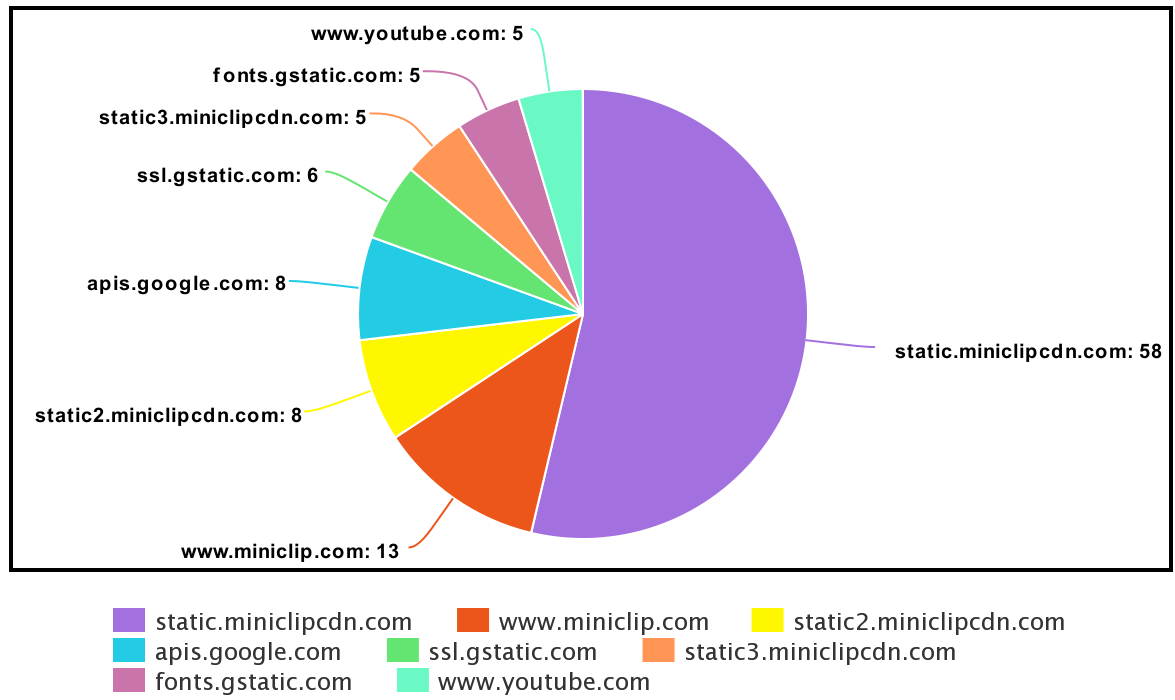
\includegraphics[width=0.45\textwidth]{res/imgs/domains.png}
    \caption{Resources domains}
    \label{fig:resdom}
\end{figure}

\subsection{Resources types}
\label{sub:res}

As seen on the Figure \ref{fig:resdom}, 57\% of the data loaded is mp4. It is due to a single video that is shown to present a game. The rest is essentially images and JavaScript, this is perfectly normal, the website has to show the preview of games and have to redirect the client if he clicks on a game.

\begin{figure}[h!]
    \centering
    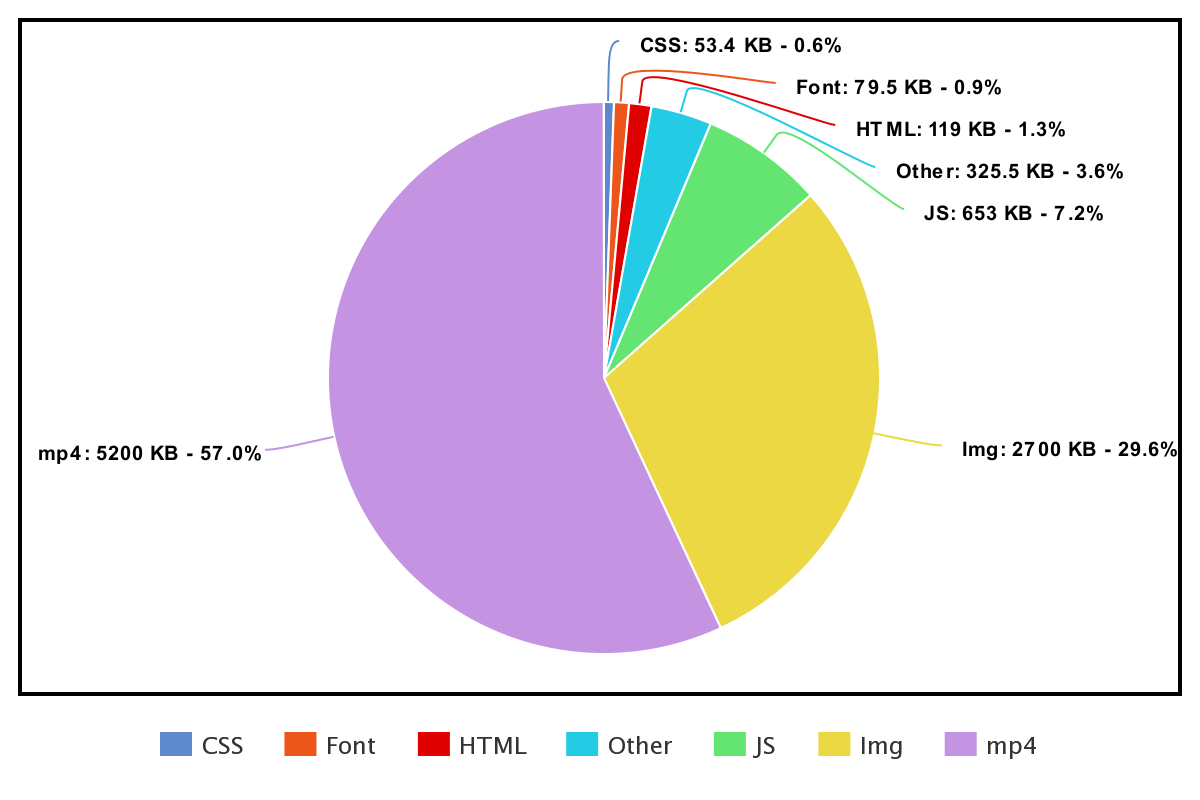
\includegraphics[width=0.45\textwidth]{res/imgs/resources.png}
    \caption{Resources types}
    \label{fig:res}
\end{figure}

\subsection{Cookies}
\label{sub:cookies}

\subsubsection{Types}

There are a lot of cookies used to track the client along all the website. They can be set by \textit{miniclip} itself or other website when request are made (IFrame or JS). There are cookies for advertisment that are set in normal mode or 'incognito' mode (\texttt{$\_\_$gads} is a Google cookie preventing the same ads from being shown to the client too many times, \texttt{$\_$fbp} is a Facebook cookie used too set third-party advertisement,...). There are cookies for identifying the client (). There are also cookies about client information such as localisation, language, ... (\texttt{$\_$country$\_$code} is used to indentify the client country, \texttt{$\_$eu$\_$cookie} is used to identfy if the client is in Europe, \texttt{$\_$language$\_$code} is used to identify the language that has to be chosen by the server, ...)

\subsubsection{Weird behavior}

When the client load the website free from cookies (First time or in incognito tab), \texttt{$\_\_$gads} and \texttt{$\_$fbp} cookies don't appear anywhere, that means that they are not set anywhere when the ressources are loaded. In fact, they are set from a \textit{JavaScript} file,the \texttt{$\_\_$gads} cookie is set in the Javascript contained in \url{https://securepubads.g.doubleclick.net/gpt/pubads_impl_modern_2019112101.js} the \texttt{$\_$fbp} cookie is set in \url{https://connect.facebook.net/signals/config/1451566791782906?v=2.9.14&r=stable}.
% On \textit{miniclip}, there are 4 different cookies owners: \textit{miniclip, google, youtube} and \textit{facebook}.
% \begin{itemize}
%     \item[--] \textbf{miniclip}
%     \begin{itemize}
%         \item \texttt{\_country\_code, \_eu\_cookie} : Contain localisation informations.
%         \item \texttt{\_fbp} : It is a Facebook cookie that is used for advertisment.
%         \item \texttt{\_\_ads} : It is a Google cookie that is used to not showing the client too much time same advertisments.
%     \end{itemize}
%     \item[--] \textbf{facebook}
%     If the client have already registered, he has these cookies \cite{facebook-cookies}:
%     \begin{itemize}
%         \item \texttt{act} : Tells when the user logged in.
%         \item \texttt{c\_user} : Contains the facebook login ID.
%         \item ...
%     \end{itemize}
%     When the user has open an incognito tab, these cookies are session cookies, instead, they expire in 90 days.
%     \item[--] \textbf{google}
%     \item[--] \textbf{youtube}
% \end{itemize}

\subsection{TCP Ports}
\label{sub:ports}

Every HTTPS request is established over the port 443 and every HTTP request is established over the port 80.

% \subsection{Non stantard headers}
% \label{sub:nonstandard}

% \textbf{X-Cache} signal that the server proxy has a valid copy of the page in its cache.


\subsection{Round Trip Time (RTT)}
\label{sub:rtt}

From the same computer in Louvain-la-Neuve, we obtain a RTT of 2.015 ms in average (on 33 packets). But we obtain different figures from other localisations, here are the figures : 
\begin{itemize}
    \itemsep-0.1em 
    \item United States :  0.775 ms
    \item South Korea : 1.549 ms
    \item Libramont, BE : 10.675 ms
    \item France : 26.801 ms
    \item Brazil : 206.450 ms
\end{itemize}

\subsection{Traceroute}
\label{sub:trace}

\section{DNS}
\label{sec:DNS}

% \begin{figure}
%     \centering
%     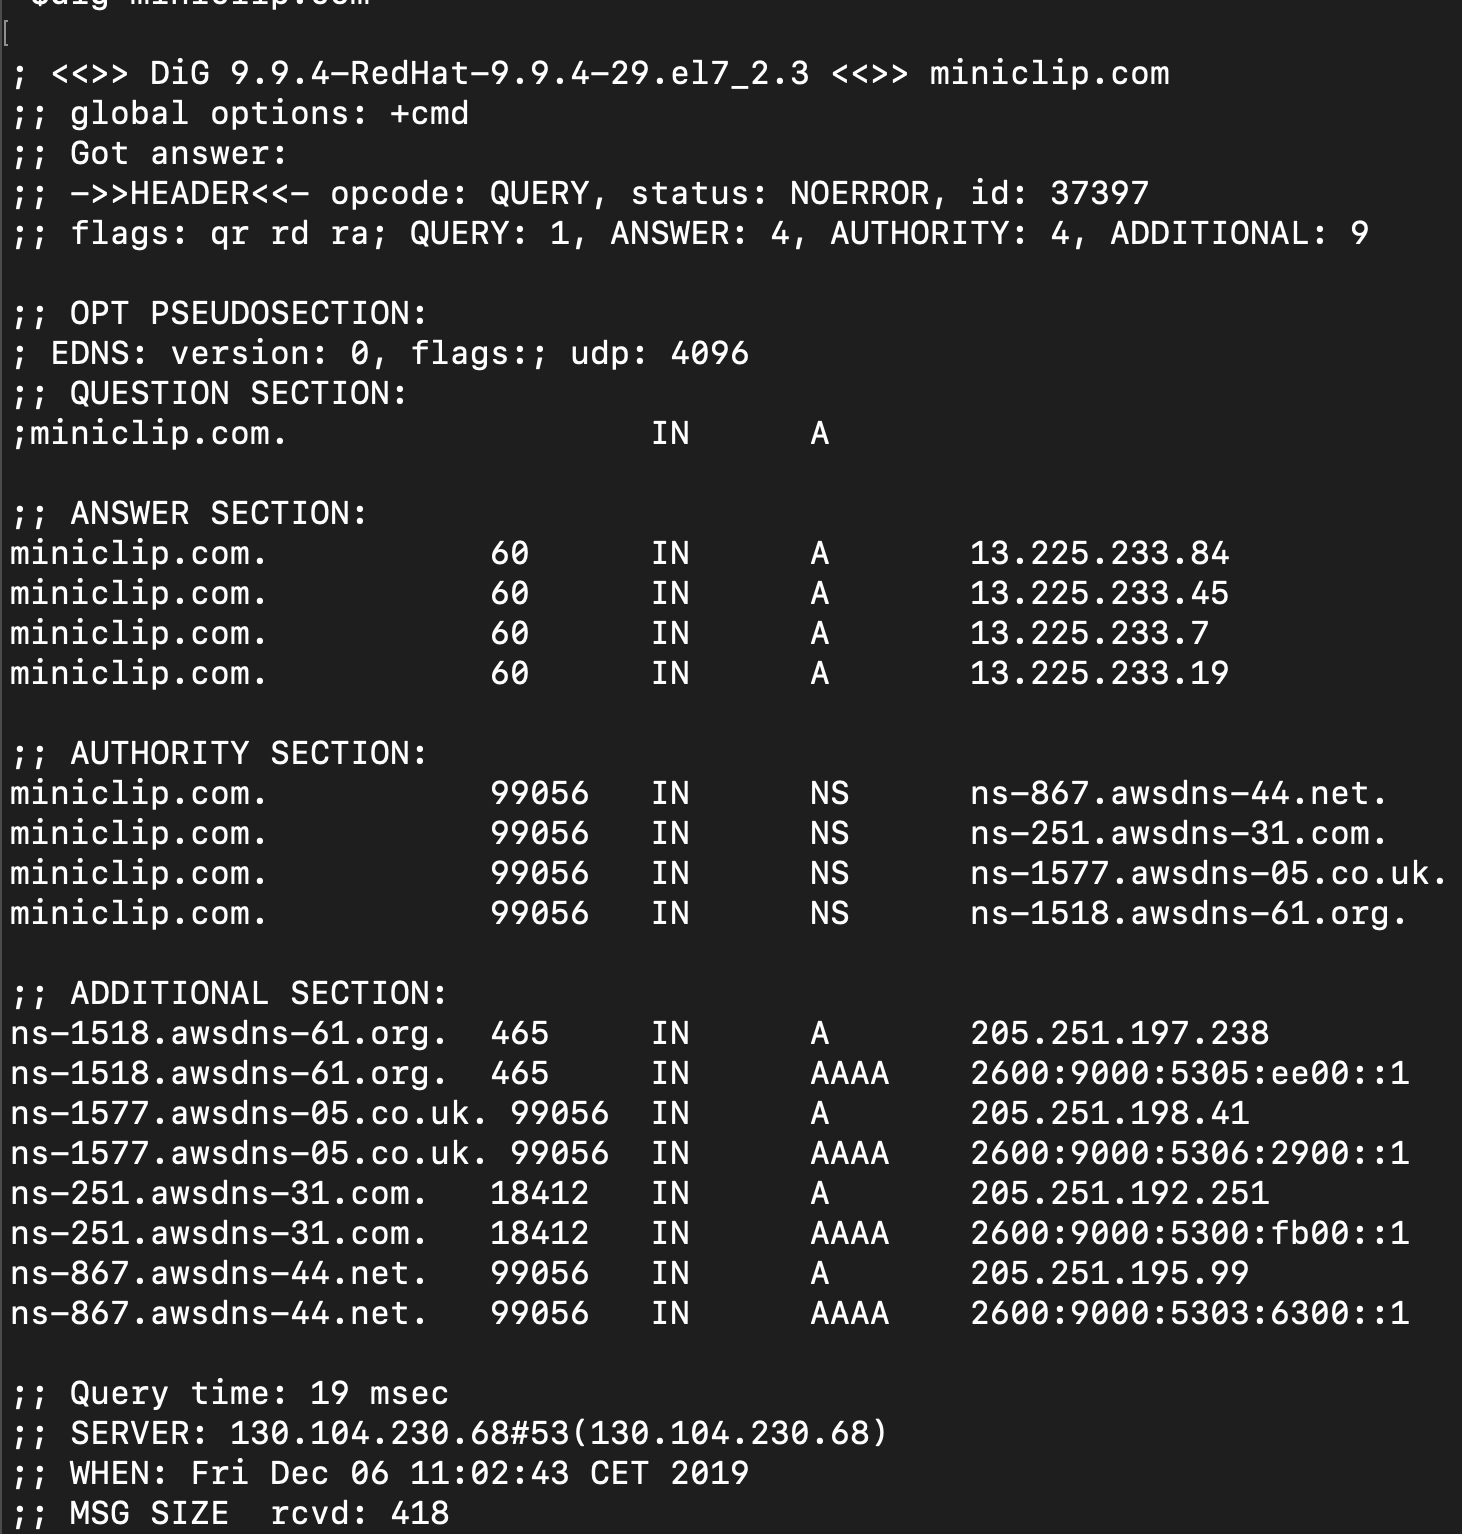
\includegraphics[width=0.45\textwidth]{Latex/res/imgs/dig.png}
%     \caption{dig miniclip.com}
%     \label{fig:dig}
% \end{figure}

For this section we will focus on the different IP adresses, the name server and the Time To Live (TTL) of each address.

\subsection{IP adresses}

\subsubsection{Explaination}
\label{subsub:ipexp}

\textit{\underline{About }}: All tests were made on the 6$^{\text{th}}$ of December 2019, in \href{https://goo.gl/maps/o6d29MMUkajAf4NXA}{Intel room} located in \href{https://goo.gl/maps/o6d29MMUkajAf4NXA}{Louvain-la-Neuve}.

\vspace{0.5cm}

Miniclip uses 4 different IPv4 addresses: 
\begin{itemize}
    \itemsep-0.1em 
    \item $13.225.233.7$
    \item $13.225.233.19$
    \item $13.225.233.45$
    \item $13.225.233.84$
\end{itemize}

To get more informations about these addresses : As seen on \textit{IP wanana} website \cite{ip}, all of these 4 addresses are hosted by \textit{Xerox Corporation} located in \href{https://goo.gl/maps/ArqaLQaFP1qYbP2j8}{Norwalk} in United-States. In fact these addresses are Content Delivery Networks (CDN), if we send a request from UK (with \url{https://gf.dev/}), we obtain 4 different addresses that have the prefix $13.35.0.0/16$ and are hosted by Amazon as we can see on the IP range file of aws \cite{awsrange}. 

So, CDN's contacted for the request depends on the localisation of the client to ensure the best speed for the client.

\subsubsection{Time To Live}
\label{subsub:ipttl}

The Time To Live of the CDN is set to 60 seconds because the best CDN may change over the network due to other users and the network bandwidth volatility (congestion, load, ...). Enabling to a good load-balancing network because it is between the client and the CDN that the most information (in term of bytes) is shared so we need a responsiveness network.

\subsection{Name servers}
\subsubsection{Explaination}
\label{subsub:nsexp}

The Name Server's (NS) used by \url{miniclip.com} are:
\begin{itemize}
    \itemsep-0.1em 
    \item ns-251.awsdns-31.com
    \item ns-867.awsdns-44.net
    \item ns-1577.awsdns-05.co.uk
    \item ns-1518.awsdns-61.org
\end{itemize}

These Name Server's are all from \textit{aws} and are located in different towns in United-States. These addresses can be reached by IPv4 or IPv6, there prefix are respectively 205.251.0.0/16 and 2600:9000::/32 .

\subsubsection{Time To Live}
\label{subsub:nsttl}

The Time To Live of these Name Servers correspondings to the domain name are set to approximatly 6 hours. And the IP addresses corresponding to the Name Servers have also a TTL of approximatly 6 hours. These TTL are pretty long because the Domain Name is pretty static so Name Servers are well set for a long time and Name Servers don't change their IP address too often. Of course it is better to refresh as much as possible but it is really expensive for the network to send request, instead each server trust its cache for the TTL.

\subsection{Extra records}
\label{subsub:extra}

For \url{miniclip.com}, we have 3 extra records that are MX, TXT and SOA.
\begin{itemize}
    \itemsep-0.1em
    \item \textbf{MX} specifies the mail server responsible for accepting email messages on behalf of a domain name \cite{mx}, here it is \url{miniclip-com.mail.protection.outlook.com} . 
    \item \textbf{TXT} is used to add extra arbitrary text over a host, readable information for a human.
    \item \textbf{SOA} (Start of Authority) is used to control zone transfers between the slave server and the master server. It also contains administrative informations.
\end{itemize}



\section{Transport Layer Security (TLS)}
\label{sec:TCP}
% Cipher Suite: TLS_ECDHE_RSA_WITH_AES_128_GCM_SHA256 (0xc02f)

To ensure the security of its clients, miniclip uses the version 1.2 of Transport Layer Security (TLSv1.2) protocol with HSTS mechanism. This protocol is used to encapsuled the information with a encryption. To trust the server, the client has to see the server's certificate.

% EXPLIQUER LES ETAPES (HANDSHAKE, TICKET, ...)

\subsection{HSTS (HTTP Strict Transport Security)}
\label{sub:hsts}

From the moment \textit{miniclip.com} has HSTS mechanism, it is only accessible using HTTPS connection and so, TLS is forced to be used. In all HTTP/2.0 answers headers, we have got \texttt{strict-transport-security: max-age=
63072000; includeSubDomains; preload}

\begin{itemize}
    \itemsep -0.1em
    \item \textbf{max-age} is the time, in seconds, that the browser should remember that a site is only to be accessed using HTTPS.
    \item \textbf{includeSubDomains} tells that this rule applies to all of the site's subdomains as well.
    \item \textbf{preload} is using to preload a list that contains domains names that by default support HSTS.
\end{itemize}

\subsection{Certificate}
\label{sub:certificate}

It is a X.509v3 certificate.

\subsubsection{Issuer}
The server's certificate is issued by Amazon (AIA: \url{http://crt.sca1b.amazontrust.com/sca1b.crt}). This certificate is used on the domain (miniclip.com) and all subdomains.

Certifcates have hierarchical authorities, the most important is the root, here, we have got :

\[
    \begin{array}{c}
        \text{miniclip.com}\\\text{(End-user)}
    \end{array}
    \xrightarrow[]{\text{issuer}}
    \begin{array}{c}
        \text{Amazon}\\\text{(Intermediate)}
    \end{array}
    \xrightarrow[]{\text{issuer}}
    \begin{array}{c}
        \text{Amazon Root CA}\\\text{(Intermediate)}
    \end{array}
\]

\[    
    \xrightarrow[]{\text{issuer}}
    \begin{array}{c}
        \text{Starfield Services Root Certificate Authority}\\\text{(Intermediate)}
    \end{array}
\]

\[     
    \xrightarrow[]{\text{issuer}}
    \begin{array}{c}
        \text{Starfield Technologies, Inc.}\\\text{(Root)}
    \end{array}
\]

As seen on \href{https://www.ssllabs.com/ssltest/analyze.html?d=miniclip.com&s=99.84.224.21}{SSLabs}, we can see that the handshake works with a lot of browser.


\subsubsection{Encryption/Decryption}
It uses \texttt{SHA-256 with RSA Encryption}.

SHA-256 is used to hash the message, it is a unilateral hash algorithm and it produces a 256 bits message.

RSA (Rivest–Shamir–Adleman) is a cryptosystem based on a pair of private and public keys. The public key is shared to everyone and is used to encrypt message. The private key is used to decrypt the message and is unique, it is kept secret.


\subsubsection{Validity}

On the 7$^{\text{th}}$ of December 2019, the certificate of miniclip.com is available until 3$^{\text{rd}}$ of October 2020, 12 am. The more the Certificat Authority is important the more the validity is long because the CA is more reliable.


% References should be produced using the bibtex program from suitable
% BiBTeX files (here: strings, refs, manuals). The IEEEbib.bst bibliography
% style file from IEEE produces unsorted bibliography list.
% -------------------------------------------------------------------------
\bibliographystyle{res/bib/IEEEbib}
\bibliography{res/bib/strings,res/bib/refs,res/bib/fields}

\end{document}
